\begin{center}
    \textsf{З А Д Ч Н И К\hspace{0.3cm}«К В А Н Т»}
\end{center}
\begin{multicols}{2}
\textit{доказать, что точки $C$ и $D$ лежат по разные стороны от точки $A$.)}
Пусть $N_1$ -- точка, симметричная точке $N$ относительно $K$ (см. рисунок). Тогда $\triangle KCN_1 = \triangle KDN$, поэтому
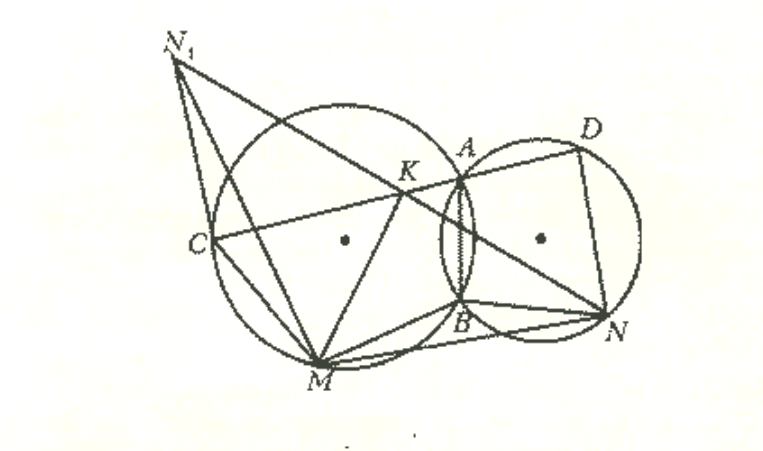
\includegraphics[width=0.5\textwidth]{pic1}
$CN_1 = ND$ и $\angle N_1CK = \angle NDK = \pi - \angle ABN$. Заметим еще, что $\angle MCK = \pi - \angle ABM$. Складывая равенства, находим, что $\angle N_1CM = \angle MBN$. Кроме того, из условия следует, что $CM = MB$ и $BN = ND$(т.е. $BN = CN_1$). Значит, $\triangle MCN_1 = \triangle MBN$, откуда $MN_1 = MN$. Отрезок $MK$ -- медиана в равнобедренном треугольнике $MNN_1$, поэтому $\angle MKN = 90\degree$.\\ \textit{Замечаение.} Задача имеет много других решений. Например, можно воспользоваться подобием треугольников $MEK$ и $KFN$, где $E$ и $F$ -- середины отрезков $BC$ и $BD$ соответственно. Эти треугольники имеют две пары взаимно перпендикулярных сторон: $EK$ и $FN$, $ME$ и $KF$; следовательно, перпендикулярны и их третьи стороны.\\Кроме того, соображения, использующие композицию поворотов, позволяет отказаться от дополнительного условия в задаче(о том, что точки $C$ и $D$ лежат по разные стороны от $A$), которое было задано лишь затем, чтобы избежать разбора различных случаев. Действительно, рассмотрим композицию поворотов\\$R_\textscn M^\beta \circ R_\textscn N^\alpha = Z_x$ -- центральная симметрия относительно некоторой точки $X$. Но \[Z_X(D) = (R_\textscn M^\beta \circ R_\textscn N^\alpha) = R_\textscn M^\beta(B) = C,\] поэтому $X$ -- середина отрезка $CD$, т.е. точка $K$. Если $N_1 = Z_K(N)$, то $N_1 = (R_\textscn M^\beta \circ R_\textscn N^\alpha)(N) = R_\textscn M^\beta(N)$, т.е. $\triangle NMN_1$ равнобедренный и $\angle MKN = 90\degree$.
\begin{flushright}
\textit{Д.Терешин}
\end{flushright}
\textsf{\textbf{M1612*.}} 
\textit{В клетках таблицы $10\times10$ расставлены числа 1, 2, 3, \dots, 100 так, что сумма любых двух соседних чисел не превосходит $S$. (Числа называются соседними, если они стоят в клетках, имеющих общую сторону.)}\\\textsf{Ответ.} 106. Пример расстановки, для которой $S = 106$, приведен на рисунке (этот пример, где наибольшие числа в "черных" клетках соседствуют с наименьшими в "белых"). Докажем теперь, что $S \geq 106$ для любой расстановки чисел в таблице. Нам понадобится следующая лемма.\\\textsf{Лемма.} \textit{Если в прямоугольнике $2\times10$ отмечено $1 \leq n \leq 9$ попарно несоседних клеток, то число неотмеченных клеток прямоугольника, соседних с отмеченными, больше n.}\\\textsf{Доказательство.} В каждом из 10 прямоугольничков $1\times2$, длинные стороны которых параллельны коротким сторонам прямоугольника $2\times10$, отмечено не более одной клетки. Если одна клетка в таком прямоугольнике отмечена, то другая -- неотмеченная, соседняя с отмеченной. Тем самым мы уже имеем $n$ та-
\begin{center}
\begin{tabular}{ |c|c|c|c|c|c|c|c|c|c| } 
 \hline
 46 & 55 & 47 & 54 & 48 & 53 & 49 & 52 & 50 & 51 \\ \hline
 60 & 41 & 59 & 42 & 58 & 43 & 57 & 44 & 56 & 45 \\ \hline
 36 & 65 & 37 & 64 & 38 & 63 & 39 & 62 & 40 & 61 \\ \hline
 70 & 31 & 69 & 32 & 68 & 33 & 67 & 34 & 66 & 35 \\ \hline
 26 & 75 & 27 & 74 & 28 & 73 & 29 & 72 & 30 & 71 \\ \hline
 80 & 21 & 79 & 22 & 78 & 23 & 77 & 24 & 76 & 25 \\ \hline
 16 & 85 & 17 & 84 & 18 & 83 & 19 & 82 & 29 & 81 \\ \hline
 90 & 11 & 89 & 12 & 88 & 13 & 87 & 14 & 86 & 15 \\ \hline
 6 & 95 & 7 & 94 & 8 & 93 & 9 & 92 & 10 & 91 \\ \hline
 10 & 1 & 99 & 2 & 98 & 3 & 97 & 4 & 96 & 5 \\ \hline
\end{tabular}
\end{center}
ких клеток, а поскольку $n \leq 9$, то (при $n \geq 1$) найдется, очевидно, и клетка, принадлежащая прямоугольничку $1\times2$ без отмеченных клеток, граничащая с отмеченной клеткой соседнего прямоугольничка $1\times2$. Следовательно, общее число неотмеченных клеток, соседних с отмеченными, больше $n$, что и требовалось доказать.\\Допустим, что $S \leq 105$ для некоторой расстановки чисел. Стерев все числа в таблице, будем вписывать их на прежние места, начиная с числа 100, в порядке убывания.\\Выделим в таблице пять неперекрывающихся горизонтальных полос размерами $10\times2$ клеток и пять неперекрывающихся вертикальных полос $2\times10$ клеток. Зафиксируем число $n_0$, после вписывания которого впервые либо в каждой горизонтальной, либо в каждой вертикальной полосе окажется не меньше одного вписанного числа; соответствующий момент назовем критическим. Пусть уже вписаны 33 числа от 100 до 68, но есть пустые горизонтальные и вертикальные полосы. Те 64 клетки таблицы, которые не входят в эти полосы, можно разбить на 32 прямоугольничка $1\times2$, хотя суммой не меньше чем $68 + 69 \textgreater 105$. Отсюда следует, что $n_0 \geq 68$.\\Заметим, что в критический момент в каждую из полос вписано не меньше 10 чисел (если бы нашлась, например, горизонтальная полоса, в которую вписано не меньше 10 чисел, то перед вписыванием числа $n_0$ в ней было бы не меньше 9 чисел, в силу чего в каждой из вертикальных полос было бы минимум по одному числу, что противоречит определению числа $n_0$). Поэтому к полосам того направления, в которых в критический момент оказалось хотя бы по одному числу, можно пременить лемму.\\Поскольку в критический момент в таблицу вписано $100 - n_0$ чисел, из леммы следует, что у клеток, куда
\end{multicols}
\newpage
На случай, если формулы из статьи не были достаточно сложными, приведу определение предела
\[\lim_{n\to\infty}x_n = A \Leftrightarrow \forall \varepsilon > 0  \exists N(\varepsilon) \in \mathbb{N} : \forall n > N(\varepsilon),  \lvert x_n - A\rvert < \varepsilon\]
Исходники: 
\url{https://github.com/naumovpavel/ITMO/tree/main/Inf/Lab6} 
